\documentclass[titlepage]{article}
\usepackage[parfill]{parskip}
\usepackage[utf8]{inputenc}
\usepackage{float}
\usepackage{graphicx}
\graphicspath{ {./graphs/} }

\title{Computer Science 2XC3 Lab 4/5}
\author{Gregory Archer, Will Clubine, Gaurav Sharma}
\date{February 8th 2023}

\begin{document}

\maketitle
\tableofcontents
\listoffigures

\newpage

\section{Executive Summary}
\begin{itemize}
    \item Experiment 1 showed that
    \item Experiment 2 showed that
\end{itemize}

\section{Part 1}

\subsection{Experiment 1}

Experiment 1 examines the probability of a graph containing cycles as the number of edges increases.

The probability of the graph containing a cycle was computed by generating 500 random graphs containing $e$ edges, alongside $n$ nodes, and observing how many were cyclical.

We completed this process for graphs containing 5, 10, 15 and 20 nodes, with the proportion of edges varying from 0\% to 120\%, with increments of 20\%.

The result is graphed in Figure 1 below

\begin{figure}[H]
    \centering
    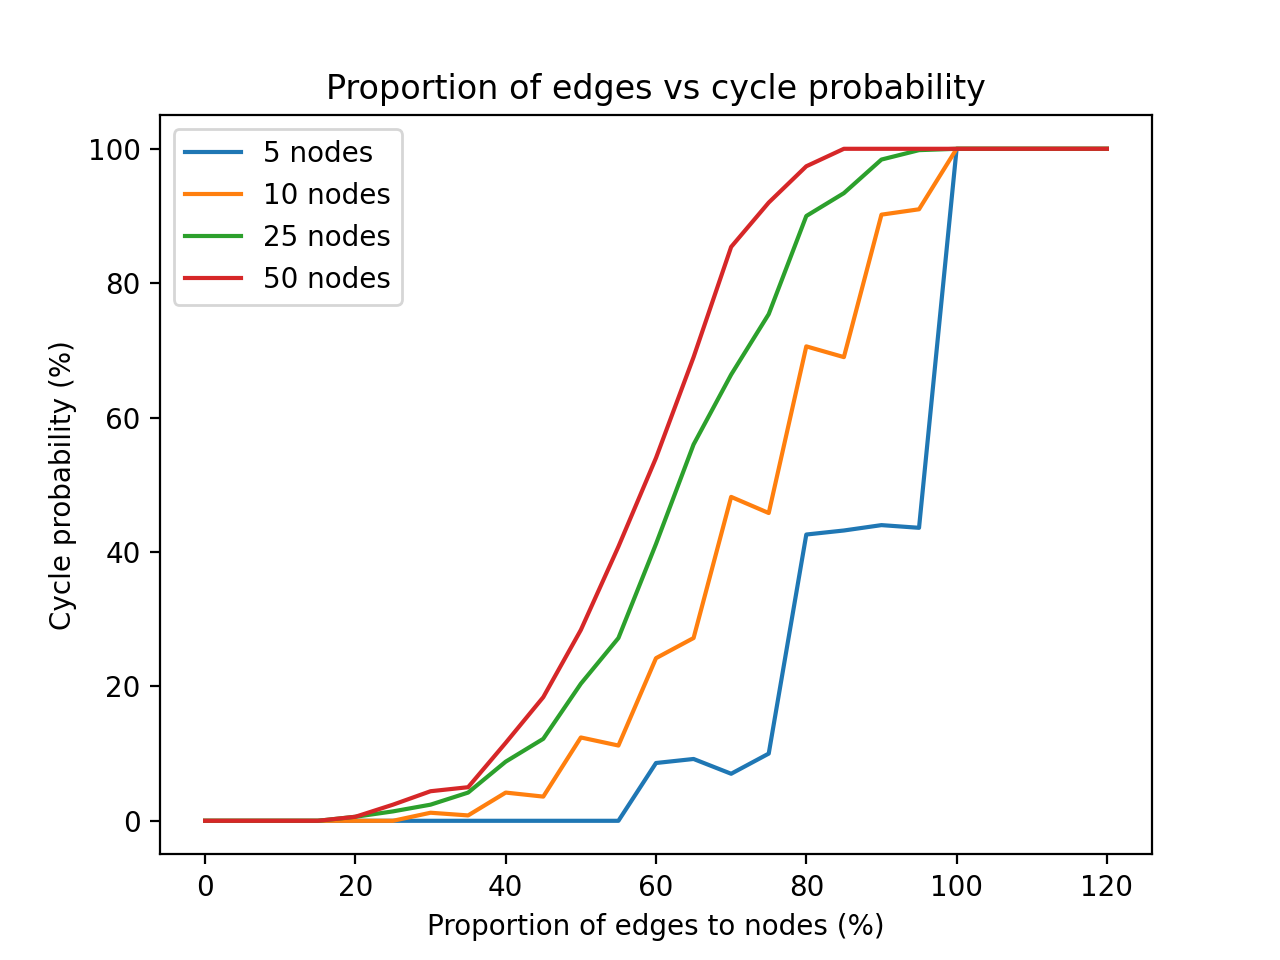
\includegraphics[width=0.8\linewidth]{experiment_1.png}
    \caption{Proportion of edges vs cycle probability}
    \label{fig:edges_vs_cycle}
\end{figure}

We have concluded from our results that as proportion of edges relative to the number of nodes increases, the cyclical probability grows, ultimately showing a direct correlation. As the number of nodes increases, the probability of a graph containing a cycle - with the same relative proportions - increases, showing another direct correlation

Additionally, once the proportion of edges to nodes is slightly beyond 100\%, there will be a graph in the cycle, regardless of the number of nodes. This is expected as any graph with more edges than nodes must contain a cycle.

\subsection{Experiment 2}

Experiment 2 examines the probability of a graph being connected as the proportion of edges to nodes increases.

We compute the approximate connected probability for a graph of $e$ edges and $n$ nodes by generating 500 random graphs with $e$ edges and $n$ nodes and determining what percentage of those graphs are connected.

This process is conducted for graphs with 5, 10, 25, and 50 nodes at different proportions of edges. Specifically, we start with 0 edges and gradually increase to 500\% the node count in 20\% increments. The result is then graphed as shown in Figure \ref{fig:edges_vs_connected} below.

\begin{figure}[H]
    \centering
    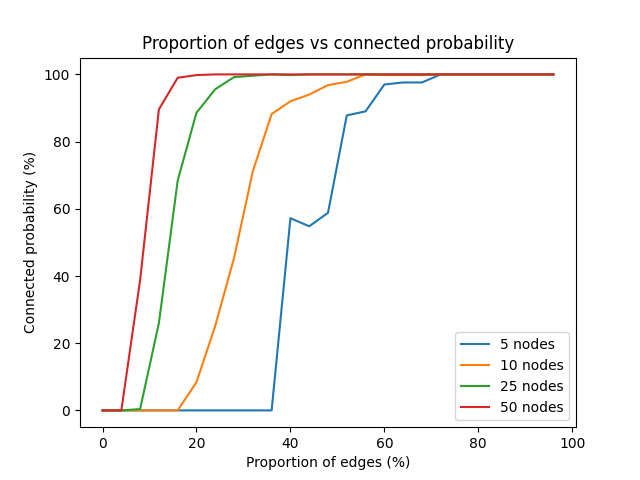
\includegraphics[width=0.8\linewidth]{experiment_2.png}
    \caption{Proportion of edges vs connected probability}
    \label{fig:edges_vs_connected}
\end{figure}

% this is wrong v will rewrite

% As seen in Figure \ref{fig:edges_vs_connected}, each graph size sits at a 0\% chance of connectedness before rapidly increasing and eventually reaching a 100\% probability of being connected; but the transitions take place at different edge proportions.

% This is because the number of edges required to make connectedness possible grows linearly with the number of nodes, while the maximum number of unique edges grows quadratically. Specifically, an undirected graph of $n$ nodes with no self-loops requires only $n - 1$ unique edges to make connectedness possible, but can have a maximum of $\frac{(n - 1) \cdot n}{2}$ unique edges.

\section{Part 2}

\subsection{Minimum Vertex Cover Approximation}

\subsubsection{Experiment 1}



\subsubsection{Experiment 2}



\subsubsection{Experiment 3}



\subsection{Maximum Independent Sets}

\begin{figure}[H]
    \centering
    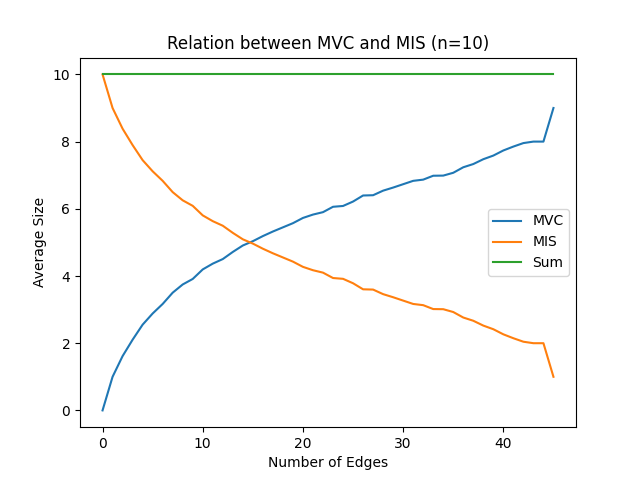
\includegraphics[width=0.8\linewidth]{mvc_mis.png}
    \caption{Relation between MVC and MIS}
    \label{fig:mvc_mis}
\end{figure}

\appendix
\section{Navigating the Code}

\begin{itemize}
    \item Each experiment in Part 1 can be found within it's own file titled \verb|experiment_#.py|
    \item Approximation experiments can be found within \verb|approximation_experiments.py|
    \item Maximum independent set experiments can be found within \verb|independent_sets.py|
    \item Additional graph functions were added to \verb|graph.py|
\end{itemize}

\end{document}
